\documentclass[tikz,border=4pt]{standalone}
\usepackage{amsmath}
\usetikzlibrary{arrows.meta,positioning}
\definecolor{ink}{HTML}{21324A}
\definecolor{vision}{HTML}{E1F1F8}
\definecolor{textbranch}{HTML}{F0E8F7}
\definecolor{learned}{HTML}{FBEDDB}

\begin{document}
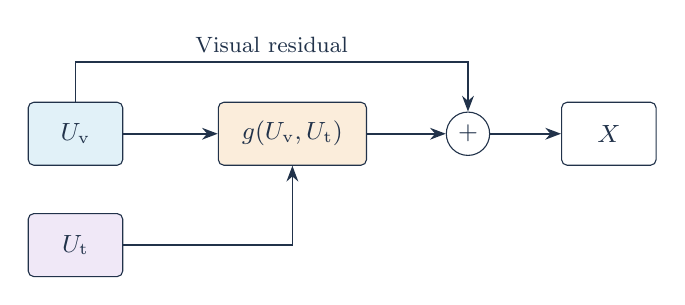
\begin{tikzpicture}[
  font=\small, text=ink,
  flow/.style={-{Stealth[length=2mm]}, draw=ink, semithick},
  block/.style={rounded corners=2pt, draw=ink, minimum height=8mm,
    minimum width=12mm, inner xsep=3mm, align=center},
  operator/.style={circle, draw=ink, inner sep=0pt, minimum size=5.5mm}
]
\node[block, fill=vision] (visual) {$U_{\mathrm v}$};
\node[block, fill=textbranch, below=6mm of visual] (text) {$U_{\mathrm t}$};
\node[block, fill=learned, right=12mm of visual] (gate) {$g(U_{\mathrm v},U_{\mathrm t})$};
\node[operator, right=10mm of gate] (sum) {$+$};
\node[block, right=9mm of sum] (output) {$X$};

\draw[flow] (visual) -- (gate);
\draw[flow] (text.east) -| (gate.south);
\draw[flow] (gate) -- (sum);
\draw[flow] (visual.north) -- ++(0,5mm)
  -| node[pos=0.25, above, font=\footnotesize] {Visual residual} (sum.north);
\draw[flow] (sum) -- (output);
\end{tikzpicture}
\end{document}
